%\title{Презентация на защите}
\documentclass[9pt,pdf,utf8,russian]{beamer}

\usetheme[progressbar=frametitle]{metropolis}
\usepackage{appendixnumberbeamer}

\usepackage{booktabs}
\usepackage[scale=2]{ccicons}

\usepackage{pgfplots}
\usepgfplotslibrary{dateplot}

\usepackage{xspace}
\newcommand{\themename}{\textbf{\textsc{metropolis}}\xspace}

\usepackage[utf8]{inputenc}

\usepackage{amssymb,amsmath}
\usepackage[utf8]{inputenc} 
\usepackage{mathrsfs}
\usepackage[matrix,arrow,curve]{xy}

\title{Метрическая и топологическая проективность, инъективность и плоскость банаховых модулей}
%\subtitle{A modern beamer theme}
\author{Немеш Норберт Тиборович}
\date{23 декабря 2016 г.}
\institute{МГУ имени М.В. Ломоносова}
% \titlegraphic{\hfill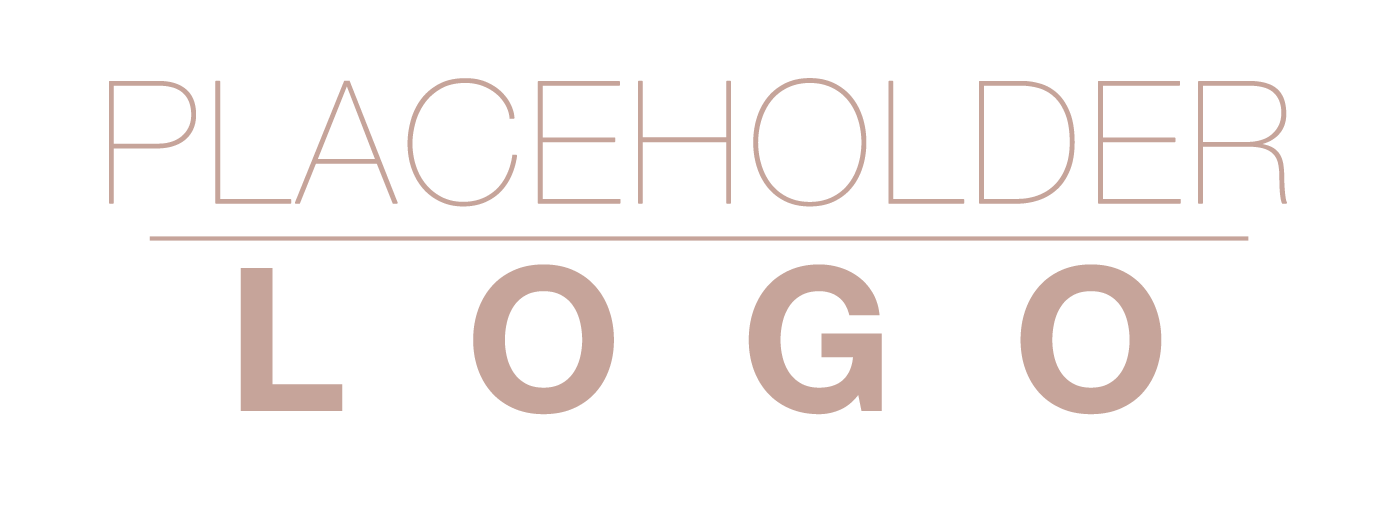
\includegraphics[height=1.5cm]{logo.pdf}}
\begin{document}

\maketitle

\section{Определения}

\begin{frame}[fragile]{Проективность}
  \begin{block}{} 
    Банахов $A$-модуль $P$ называется \textit{проективным}, если для любого \alert{допустимого} 
    эпиморфизма $\xi:X\to Y$ и любого морфизма $\phi:P\to Y$ существует морфизм $\psi:P\to X$  делающий диаграмму 
    \begin{table}
      \begin{tabular}{cc}
        $\xymatrix{
        & {X} \ar[d]^{\xi}\\
        {P} \ar@{-->}[ur]^{\psi} \ar[r]^{\phi} &{Y}}$
        &
        \alert<2>{\only<2>{$\Vert\phi\Vert=\Vert\psi\Vert$}}\\
      \end{tabular}
    \end{table}
    коммутативной.
  \end{block}

  \pause

  Какие эпиморфизмы считать допустимыми?

  \begin{itemize}[<+- | alert@+>]
    \item Метрическая теория: $\xi$ --- строгая коизометрия, т.е. $\xi(B_X)=B_Y$
    \item Топологическая теория: $\xi$ --- открытое отображение
    \item Относительная теория: $\xi$ имеет дополняемое ядро
    \end{itemize}
\end{frame}

\begin{frame}[fragile]{Инъективность}
  \begin{block}{} 
    Банахов $A$-модуль $J$ называется \textit{инъективным}, если для любого \alert{допустимого} 
    мономорфизма $\xi:Y\to X$ и любого морфизма $\phi:Y\to J$ существует морфизм $\psi:X\to J$  делающий диаграмму 
    \begin{table}
      \begin{tabular}{cc}
        $\xymatrix{
        & {X} \ar@{-->}[dl]_{\psi} \\
        {J} &{Y} \ar[l]_{\phi} \ar[u]_{\xi}}$
        &
        \alert<2>{\only<2>{$\Vert\phi\Vert=\Vert\psi\Vert$}}\\
      \end{tabular}
    \end{table}
    коммутативной.
  \end{block}
  \pause
  
  Какие мономорфизмы считать допустимыми?

  \begin{itemize}[<+- | alert@+>]
    \item Метрическая теория: $\xi$ --- изометрия
    \item Топологическая теория: $\xi$ --- вложение с замкнутым образом
    \item Относительная теория: $\xi$ имеет дополняемый образ
  \end{itemize}
\end{frame}

\begin{frame}{Плоскость}
  \begin{block}{} 
  	Банахов $A$-модуль $F$ называется \textit{плоским}, если модуль $F^*$ инъективен.
  \end{block}
\end{frame}

\begin{frame}{Гомологическая теория банаховых пространств}
  \begin{itemize}
  \item Метрическая инъективность (Kelly, Nachbin, Goodner, Hasumi 1950-1958)
  \item Метрическая плоскость (Grothendieck, 1955)
  \item Топологическая проективность (Köthe, 1966)
  \item Топологическая плоскость (Retherford, 1972)
  \end{itemize}
\end{frame}

\section{Основные результаты}

\begin{frame}{Проективные идеалы}
  \begin{alertblock}{Теорема} 
    Замкнутый идеал коммутативной банаховой алгебры, обладающий ограниченной аппроксимативной 
    единицей топологически проективен тогда и только тогда, когда он обладает единицей.
  \end{alertblock}
  \pause
  \begin{alertblock}{Теорема} 
    Замкнутый идеал коммутативной банаховой алгебры, обладающий \alert{сжимающей} аппроксимативной 
    единицей \alert{метрически} проективен тогда и только тогда, когда он обладает единицей \alert{нормы 1}.
  \end{alertblock}
  \pause
  \begin{alertblock}{Теорема} 
  	Замкнутый левый идеал \alert{$C^*$-алгебры} метрически или топологически проективен тогда и только тогда, когда он обладает самосопряженной правой единицей.
  \end{alertblock}
\end{frame}

\begin{frame}{Плоские модули}
  \only<1>{
    \begin{block}{Определение (Lindenstrauss-Pełczyński, 1968)} 
      Пространство $E$ называется $\mathscr{L}_p$-пространством если существует константа $C>0$ такая, что для любого конечномерного 
      подпространства $F$ в $E$ существует конечномерное подпространство $G$ в $E$ $C$-изоморфное конечномерному $\ell_p$ пространству и содержащее $F$.
    \end{block}
    \begin{exampleblock}{Пример}
      \begin{itemize}
        \item $L_1\in\mathscr{L}_1$
        \item $C(K)\in\mathscr{L}_\infty$
      \end{itemize}
    \end{exampleblock}
  }
  \pause
  \begin{block}{Определение}
 	 Банахова алгебра $A$ называется аменабельной, если все её правые, левые и двусторонние	 модули \textit{относительно} плоские.
  \end{block}
  \pause
  \begin{alertblock}{Теорема}
  	Над аменабельной банаховой алгеброй всякий банахов модуль, являющийся $\mathscr{L}_1$-пространством, топологически плоский.
  \end{alertblock}
  \pause
  \begin{block}{Теорема (J.R. Retherford, 1972)} 
  	$\mathscr{L}_1$-пространства --- это в точности топологически плоские банаховы \textit{пространства}.
  \end{block}
\end{frame}

\begin{frame}{Инъективные $C^*$-алгебры}
  \begin{block}{Определение (Dubinsky-Pełczyński-Rosenthal, 1972)}
    Говорят, что банахово пространство $E$ имеет свойство l.u.st. если $E^{**}$ изоморфно дополняемому подпространству некоторой банаховой решетки.
  \end{block}
  \pause
  \begin{alertblock}{Теорема}
    Если $C^*$-алгебра топологически инъективна как правый модуль над собой, то
    \begin{itemize}
      \item $A$ имеет свойство l.u.st;
      \item $A$ --- субоднородная $C^*$-алгебра;
      \item $A$ --- есть $*$-подалгебра в $M_n(C(K))$
    \end{itemize}
  \end{alertblock}
\end{frame}

\begin{frame}{Инъективные $AW^*$-алгебры}
  \begin{block}{Определение}
    $AW^*$ алгебра --- это $C^*$-алгебра в которой у любого подмножества правый алгебраический аннулятор порожден некоторой проекцией.
  \end{block}
  \pause
  \[
    W^*\subset AW^*\subset C^*
  \]
  \pause
  \begin{alertblock}{Теорема}
      $AW^*$-алгебра $A$ топологически инъективна как правый модуль над собой тогда и только тогда, когда 
    \[
      A=\bigoplus_{i=1}^N M_{n_i}(C(K_i)),
    \]
    где $K_i$ --- стоуновы пространства.
  \end{alertblock}
\end{frame}

\begin{frame}{Свойство Данфорда-Петтиса}
   \begin{block}{Определение (Grothendieck, 1953)}
     Говорят, что банахово пространство $E$ имеет свойство Данфорда-Петтиса, если для любого банахова пространства $F$ 
     всякий слабо компактный оператор $T:E\to F$ будет вполне непрерывным.
   \end{block}
   \pause
   \begin{exampleblock}{Пример}
    \begin{table}
      \begin{tabular}{lr}
        Обладают & Не обладают\\
        \midrule
        $L_1$, $C(K)$ & рефлексивные пространства\\
      \end{tabular}
    \end{table}
   \end{exampleblock}
   \pause
   \begin{alertblock}{Теорема}
     Если банахова алгебра является $\mathscr{L}_1$- или $\mathscr{L}_\infty$-пространством, 
     то все её топологически проективные, инъективные и плоские модули имеют свойство Данфорда-Петтиса.
   \end{alertblock}
\end{frame}

\begin{frame}{Маленькая категория}
  \alert{Итог}: большинство модулей гомологически нетривиальны.
  \pause
  
  \alert{Причина}: категория банаховых модулей очень большая.
  \pause
  \begin{exampleblock}{Пример маленькой категории}
    \[
      A=B(\Omega,\Sigma)
    \]
    \pause
    \[
      \operatorname{Ob}(\mathbf{C})=\{L_p(\Omega,\mu): 1\leq p\leq\infty, \mu \mbox{ -- }\sigma\mbox{-аддитивная мера}\}
    \]
    \pause
    \[
      \operatorname{Hom}(\mathbf{C})=\{M_g:L_p(\Omega,\mu)\to L_q(\Omega,\nu):f\mapsto gf\}
    \]
  \end{exampleblock}
  \pause
  \begin{alertblock}{Теорема}
    В категории $\mathbf{C}$ все модули являются проективными, инъективными и плоскими в смысле метрической, топологической и относительной теории.
  \end{alertblock}  
\end{frame}


\begin{frame}{Ссылки}
  \begin{itemize}
    \item Немеш Н. Метрически и топологически проективные идеалы банаховых алгебр // Матем. Заметки.  --- 2016. --- Т. 99, № 4. --- С. 526-533.
    \item Немеш Н. Топологически инъективные $C^*$-алгебры // Функц. анал. и прил. --- 2016. --- Т. 50, № 2. --- С. 88-91.
    \item Немеш Н. Гомологическая тривиальность категории модулей $L_p$ // Вест. Моск. ун-та. Сер. 1. Математика. Механика. --- 2016. Т. 71, № 4. --- С. 3---12.
  \end{itemize}
\end{frame}

% Тема моей диссертации --- ``Метрическая и топологическая проективность, инъективность и плоскость банаховых модулей''.
% Я провел исследование этих двух версий банаховой гомологии и сравнил их с классической (так называемой относительной) банаховой гомологией.
% Во всех трех теориях я изучал проективные инъективные и плоские банаховы модули. Мы будем называть их гомологически тривиальными. 

% ---------

% Определяются они так

% ---------

% Модуль $P$ называется проективным если для каждого допустимого эпиморфизма $\xi$ и любого морфизма $\phi$ должен существовать морфизм $\psi$ делающий диаграмму коммутативной

% ---------

% Какие можно взять допустимые эпиморфизмы?
% В метрической теории это строгие коизометрии, то есть операторы отображающие замкнутый единичный шар на замкнутый единичный шар. Кстати, для метрической теории мы дополнительно требуем равенство норм морфизмов $\phi$ и $\psi$.

% ---------

% В топологической это открытые отображения.

% ---------

% В относительной - отображения у которых ядро есть подпространство дополняемое в смысле банаховой геометрии.

% ---------

% В случае с инъективностью мы рассматриваем допустимые мономорфизмы и все стрелки в диаграмме меняют направление
 
% ---------

% Допустимые мономорфизмы для трех теорий соответственно изометрии,

% ---------

% вложения с замкнутым образом 

% ---------

% и вложения с дополняемым образом.

% ---------

% Во всех трех теориях плоскость мы определяем через инъективность: модуль называется плоским если сопряженный к нему инъективен

% Как видно, метрическая и топологическая банахова гомология представляют интерес потому что в них рассматриваются модули для которых разрешимы
% максимально широкие классы задач подъема и продолжения морфизмов.

% ---------

% Для случая нулевой алгебры метрическая и топологическая теория вырождается в гомологическую теорию банаховых пространств. Основные задачи в этой области были решены в середине прошлого века
% Гротендиком, Кётэ, Келли, Нахбиным, Резерфордом.

% ---------

% Перейдем к главным результатам диссертации.

% ---------

% Поиск проективных модулей естественно начать с идеалов. Здесь я доказал следующую теорему

% Замкнутый идеал {\it коммутативной} банаховой алгебры, обладающий ограниченной аппроксимативной единицей топологически проективен тогда и только тогда, когда он обладает единицей.

% ---------

% В метрическом случае надо потребовать чтобы аппроксимативная единица была сжимающая, тогда идеал будет иметь единицу нормы 1:

% Отмечу, что в относительной теории есть лишь необходимое условие проективности идеала, а именно паракомпактность его спектра.

% ---------

% В некоммутативном случае удалось получить результат для $C^*$-алгебр, а именно:

% Левый замкнутый идеал $C^*$-алгебры метрически или топологически проективен тогда и только тогда, когда он обладает самосопряженной правой единицей.

% Опять же в относительной теории известно лишь, что все идеалы сепарабельных $C^*$-алгебр проективны.

% ---------

% Чтобы сформулировать следующий результат мне нужно дать определение пространств Линденштраусса-Пельчинского.
% Пространство $E$ называется $\mathscr{L}_p$-пространством если существует константа $C>0$ такая что для любого конечномерного подпространства $F$ в $E$ 
% существует конечномерное подпространство $G$ в $E$ $C$-изоморфное конечномерному $\ell_p$-пространству и содержащее $F$.

% Грубо говоря это пространства локально устроенны как $\ell_p$-пространства.

% ---------

% Всякое пространство непрерывных функций на компакте есть $\mathscr{L}_\infty$-пространство, 
% Всякое пространство функций интегрируемых по Лебегу является $\mathscr{L}_1$ пространством

% ---------

% Еще одно определение, теперь из банаховой гомологии:

% Банахова алгебра $A$ называется аменабельной, если все ее правые, левые и двусторонние модули относительно плоские

% В некотором смысле это гомологически лучшие алгебры, и класс таких алгебр достаточно широк.

% ---------

% Итак, следующий мой результат это необходимое условие топологической плоскости банахова модуля

% Над аменабельной банаховой алгеброй всякий банахов модуль, являющийся $\mathscr{L}_1$-пространством, топологически плоский.

% ---------

% Тут, кстати, стоит напомнить результат Резерфорда: 

% Все топологически плоские банаховы пространства это в точности $\mathscr{L}_1$-пространства.

% ---------

% Перейдем к следующему примеру подтверждающему важную роль банаховой геометрии для изучения инъективности.

% Говорят, что банахово пространство $E$ имеет свойство l.u.st. если $E^{**}$ изоморфно дополняемому подпространству некоторой банаховой решетки.

% ---------

% Для меня это свойство важно потому что все $C^*$-алгебры топологически инъективные над собой как правые модули имеют свойство l.u.st. Как следствие они являются
% субоднородными, то есть могут быть представлены как инволютивные подалгебры в матричных алгебрах с коэффициентами в алгебре непрерывных функций.

% ---------

% Это было необходимое условие. 
% Критерий топологической инъективности удалось получить для $AW^*$-алгебр.
% $AW^*$ алгебра --- это $C^*$-алгебра в которой у любого подмножества правый алгебраический аннулятор порожден некоторой проекцией.
% Эти алгебры образуют промежуточный класс между 
% $C^*$-алгебрами и алгебрами фон Нойманна.

% Теперь критерий:

% $AW^*$-алгбера топологически инъективна как правый модуль над собой тогда и только тогда, 
% когда она является прямой суммой матричных алгебр с коэффициентами в коммутативных $AW^*$-алгебрах

% ---------

% Еще один пример связан со свойством Данфорда-Петтиса.

% Говорят, что банахово пространство $E$ имеет свойство Данфорда-Петтиса, если для любого банахова пространства $F$ всякий слабо компактный оператор $T:E\to F$ будет вполне непрерывным.

% ----------

% Это свойство определил Гротендик и доказал, что им обладают все $L_1$ и $C(K)$-пространства, но им не обладает ни одно бесконечномерное рефлексивное пространство.
% Я же доказал, что

% ---------

% Если банахова алгебра, является $\mathscr{L}_1$- или $\mathscr{L}_\infty$-пространством, то все ее топологически проективные, инъективные и плоские модули имеют свойство Данфорда-Петтиса.

% Отмечу, что в относительной банаховой гомологии такое необходимое условие не выполняется.

% -----------

% Из полученных результатов можно вывести (и это сделано в моей работе), что большинство классических модулей анализа не являются гомологически тривиальными ни в метрической ни в топологической теории. 

% -----------

% Причина состоит в том что эти модули рассматриваются в очень большой категории --- категории всех модулей

% -----------

% Но ситуация может кардинально измениться для маленьких категории. 
% Рассмотрим алгебру ограниченных измеримых функций на измеримом пространстве.

% -----------

% Рассмотрим категорию $C$ состоящую из $L_p$-пространств рассмотренных как модули над этой алгеброй. 

% -----------

% В этом случае морфизмы этой категории будут операторами умножения. Мне удалось описать все допустимые операторы умножения в этой категории и в итоге получился следующий результат:

% -----------

% В категории $\mathscr{C}$ все модули являются проективными, инъективными и плоскими в смысле метрической, топологической и относительной теории.

\end{document}
